\documentclass[a4,10pt,preprint]{sigplanconf}
%\usepackage[a4paper]{geometry}
\usepackage{amsmath,graphicx,epsfig}% to put in axodraw
   % pictures, use colour in the document, put your citations as [1-4]
   % rather than [1,2,3,4] (it looks nicer, and the extended LaTeX2e
   % graphics package. 
\usepackage{latexsym,amssymb,epsf} % don't remember if these are
   % needed, but their inclusion can't do any damage
\usepackage{alltt}
\usepackage{graphicx}
\date{}
\begin{document}
\conferenceinfo{Eurosys 2011}{Austria} 
\copyrightyear{2011} 
\copyrightdata{to be supplied} 

\titlebanner{banner above paper title}        % These are ignored unless
\preprintfooter{This paper describes our research  with replacing OS Bypass on Blue Gene Supercomputers.}   % 'preprint' option specified.
\authorinfo{Ronald G. Minnich\thanks{\protect
\includegraphics[height=0.3in]{thunderchicken}%
}}
           {Sandia National Laboratories}
           {rminnich@sandia.gov}
\authorinfo{Don W. Rudish}
           {Sandia National Laboratories}
           {dwrudis@sandia.gov}
\title{\Large \bf Experiments using Currying and process-private system calls as an alternative to OS Bypass}
\maketitle
\thispagestyle{empty}
\pagestyle{empty}
\subsection*{Abstract}
The cost of moving network data through the operating system kernel has been a concern for several decades. In High Performance Computing (HPC) systems, OS Bypass is used to embed a network device driver in a user-mode library such as MPI, thus bypassing the entire kernel network stack. OS Bypass, in networking, is the equivalent of graphics libraries that drive
hardware directly, instead of using the operating system. 

The development of OS Bypass support software, and its attendant Remote DMA capabilities, has consumed HPC software development for over two decades starting in the 1980s with SCRAMNet\cite{scramnet}. In the Infiniband and Ethernet communities, the perceived need for OS Bypass for multiple processes has led to the creation of virtualizing
network interfaces, new network protocols such as iWarp, and new chipset technology including IOMMUs. It has also led to its share of new security exploits as well\cite{iommubug}. 
In an interesting and ironic twist, the existence of this new and very complex software 
has resulted in a great deal of additional complexity in the kernel, and in the creation of layers of code in both user mode and the network card operating systems that reimplement much of the  bypassed kernel code. 
Correct implementation of OS Bypass, a seemingly simple idea,  is anything but simple. 

As part of our research with the Plan 9 operating system on
supercomputers such as IBM's Blue Gene systems, we have been
reconsidering the question of OS Bypass. In this paper we describe one
such experiment in which kernel drivers are able, given a system call
and a set of parameters, to create a new system call -- in essence,
Currying the arguments and function to make a new function. This new
system call is only available to the calling process, providing a
process-private system call, analogous to process-private name spaces.

Currying and process-private system calls can make a dramatic improvement in IO system call performance. In this paper we describe both positive and negative results of using this new idea, and how much more we might do in order to remove OS Bypass as a communications mechanism in HPC. 

\section{Introduction}
We have ported the Plan~9 research operating system to the IBM Blue Gene/L and /P series machines\cite{plan9bgp}, which have up to 65536 4-core Power PC 450 CPUs and several dedicated custom interconnect networks. In contrast 
to 20 years of tradition in High Performance Computing (HPC), we require that programs access these networks via
the traditional kernel read/write interface, rather than the more traditional (for HPC) OS bypass. Put another way, we are moving the device driver from the 
programs back into the OS. 

The drivers were moved into the programs in the first place, decades
ago, because the OS took too long to move data to the network. Having
programs use the kernel for I/O will only be effective if the kernel
I/O path can be greatly improved. An essential improvement is reducing
the time overhead for getting data from the program to the network for
very small packets, such as a single float or integer. While it is
not essential for all programs to have such low-latency access, it is
essential that it be available.

In this paper we discuss our modifications to  Plan~9 to support sub-microsecond "bits to the wire" (BTW) 
performance. Rather than taking the traditional approach of radical optimization of the operating system at 
every level, we apply a mathematical technique known as Currying, or pre-evaluation of functions with constant 
parameters; and add a new capability to Plan~9, namely, process-private system calls. Currying provides 
a technique for creating new functions in the kernel; process-private system calls allow us to link 
those new functions to individual processes. With these two techniques we can allow kernel drivers to provide a fast path to user programs. We replace whole-kernel optimization, which has proven ineffective, with single-driver optimization which has proven to work quite well. 

Because the Blue Gene systems and Plan~9 are unfamiliar to most, we have structured the paper as follows: we first provide an on overview of the Blue Gene system and Plan~9. We next discuss the question of OS Bypass, then describe the work we have done to provide a fast path through the kernel to the network. Finally, we discuss performance and future work. 

\subsection{Blue Gene and its operating systems}
The IBM Blue Gene\cite{DBLP:journals/ibmrd/GaraBCCCGHHHKLOSTV05} series of supercomputers, among the fastest in the world, are also unique in that they are purpose built from the chip to the system level. In contrast to other systems which use a standard off-the-shelf CPU placed on a motherboard and connected to network chips, IBM has embedded network functionality on the CPU as shown in Figure \ref{bglchip}. These CPUs are then packaged into boards which consist of little more than DRAM and a connector, and from there to full systems.The result is a greatly simplified system which, in turn, is extremely reliable; the BG/L system at Lawrence Livermore National Lab, with 128,000 CPUs, has an average uptime of 10 days. The term uptime in this case means that after 10 days, {\em everything} is still working; any failure of any subsystem, down to a single DRAM cell, counts as an interrupt.
\begin{figure}
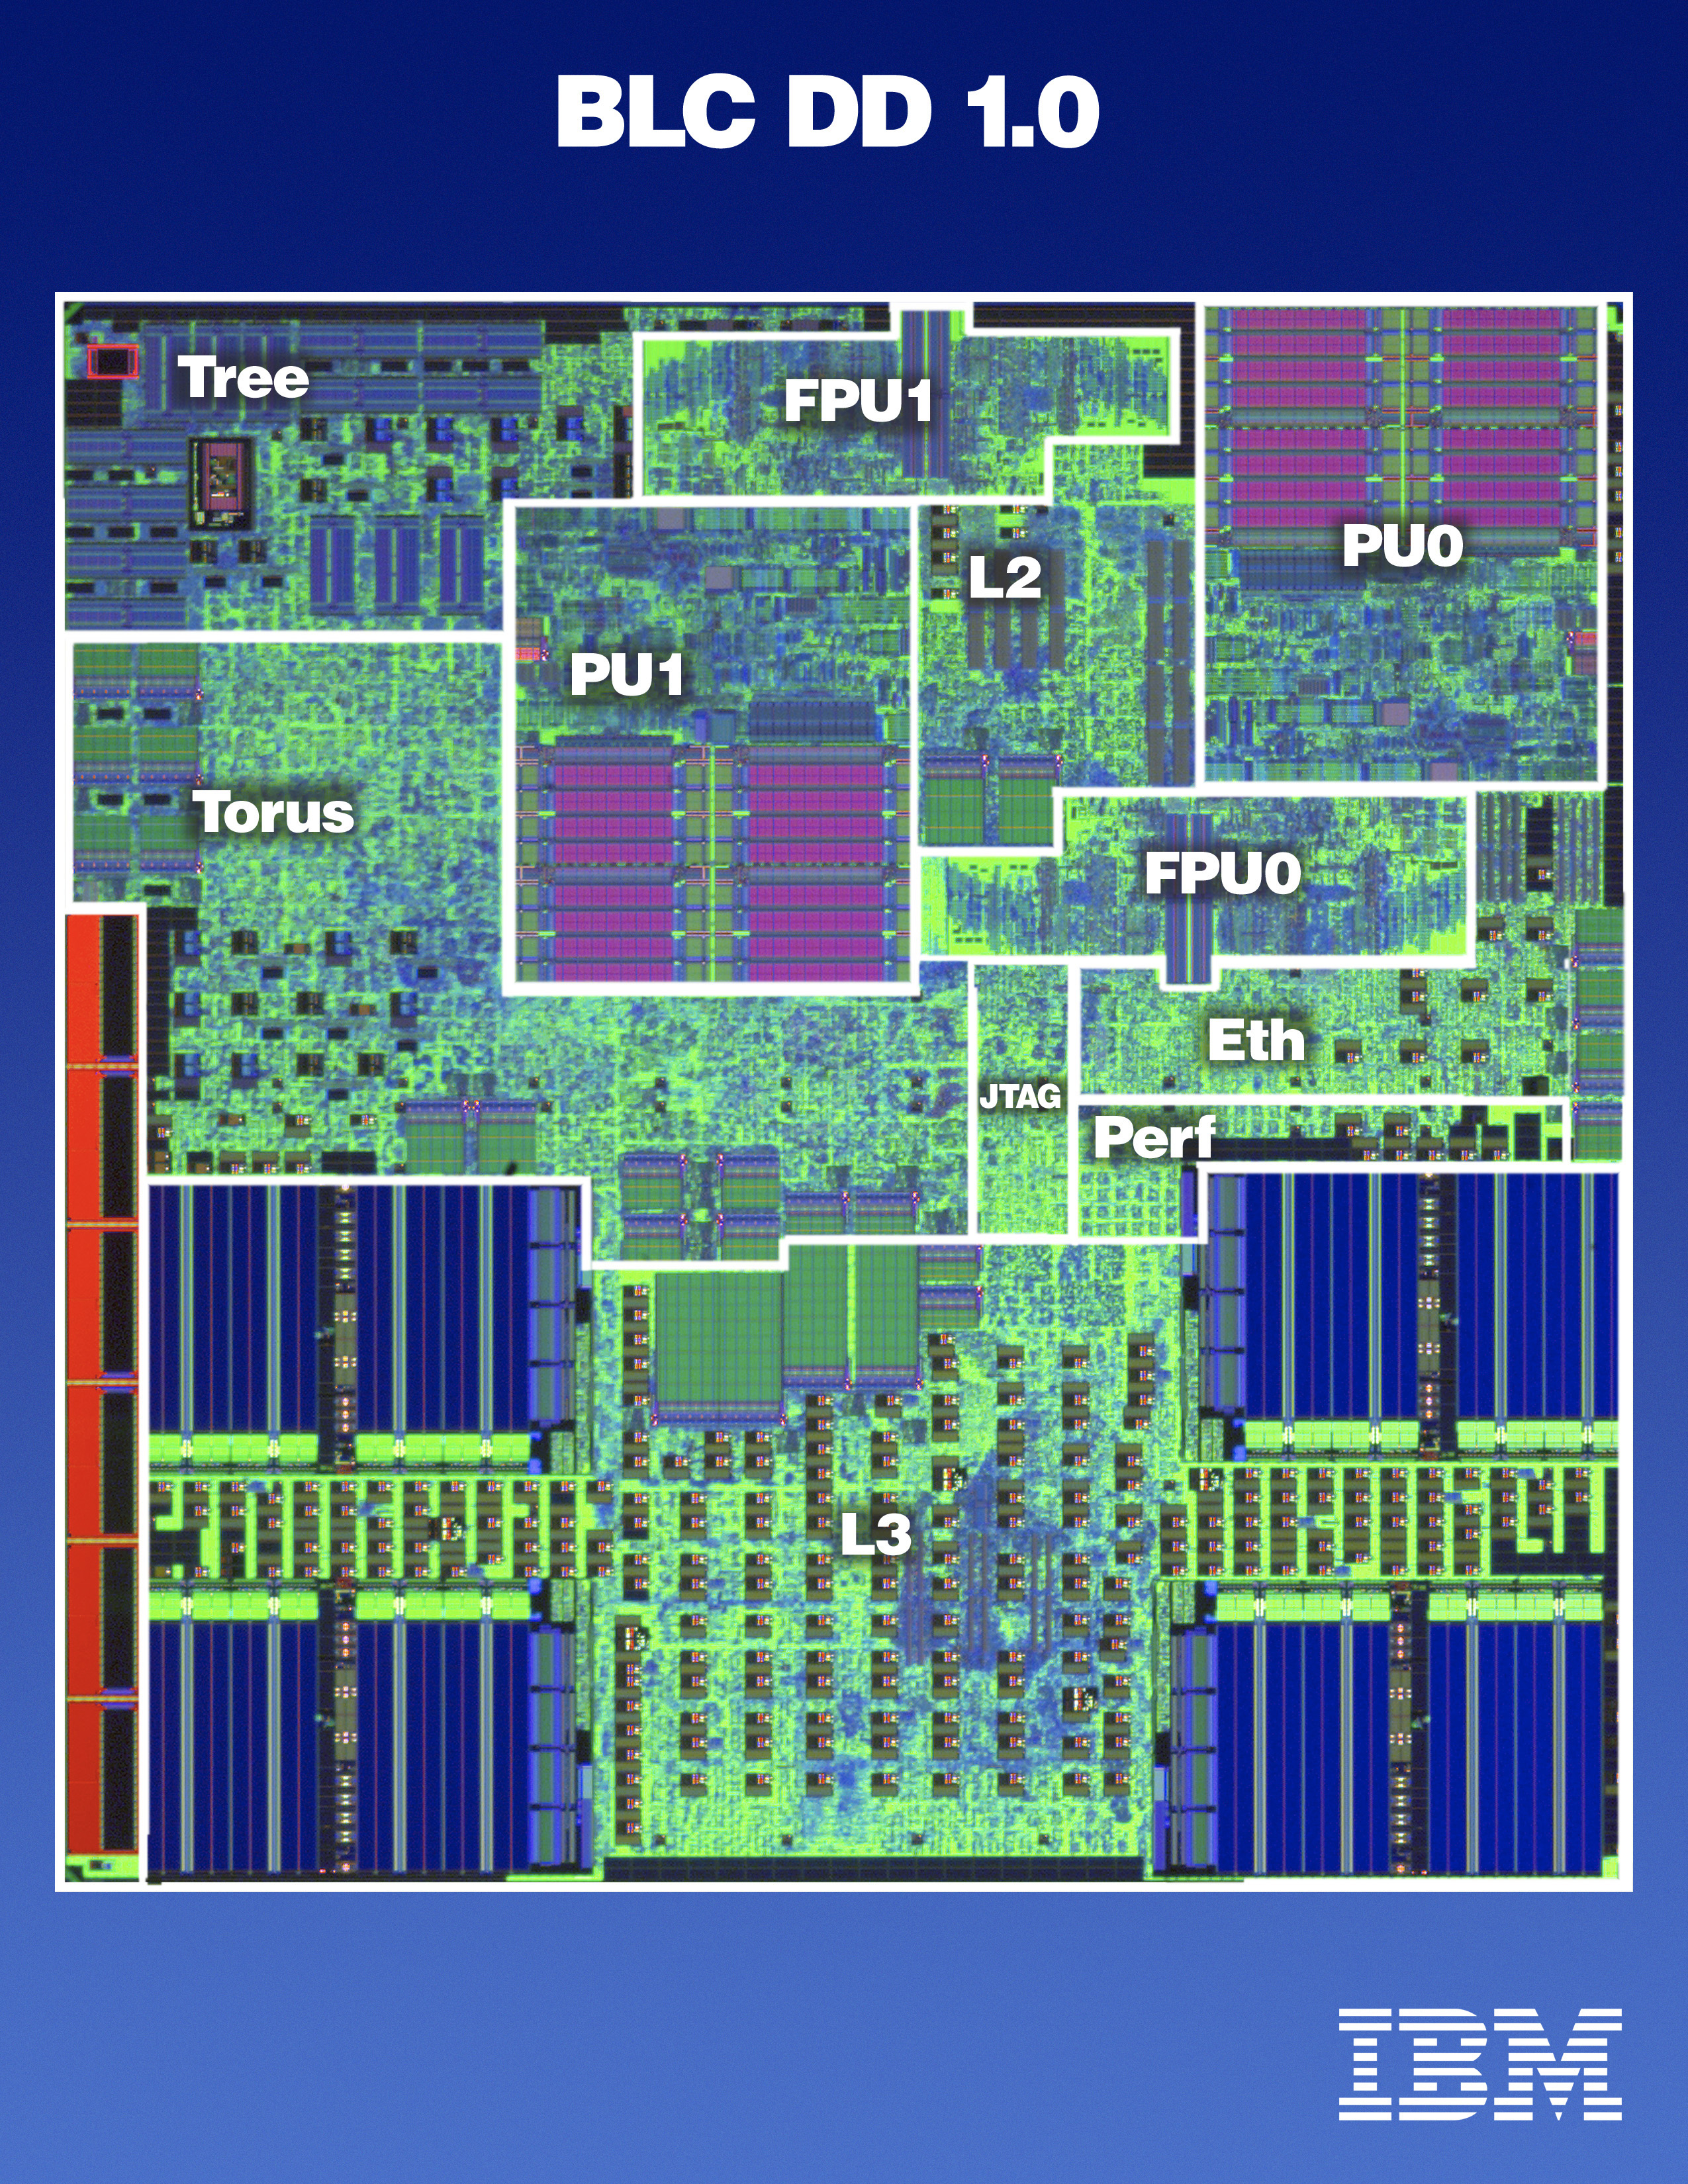
\includegraphics[width=.3\textwidth]{bglchip.eps} 
\caption{\label{bglchip}Blue Gene/L CPU showing dedicated network hardware (Torus, Tree, Eth, and JTAG). Note that on most CPUs the Eth block is not connected.}
\end{figure}
\begin{figure}
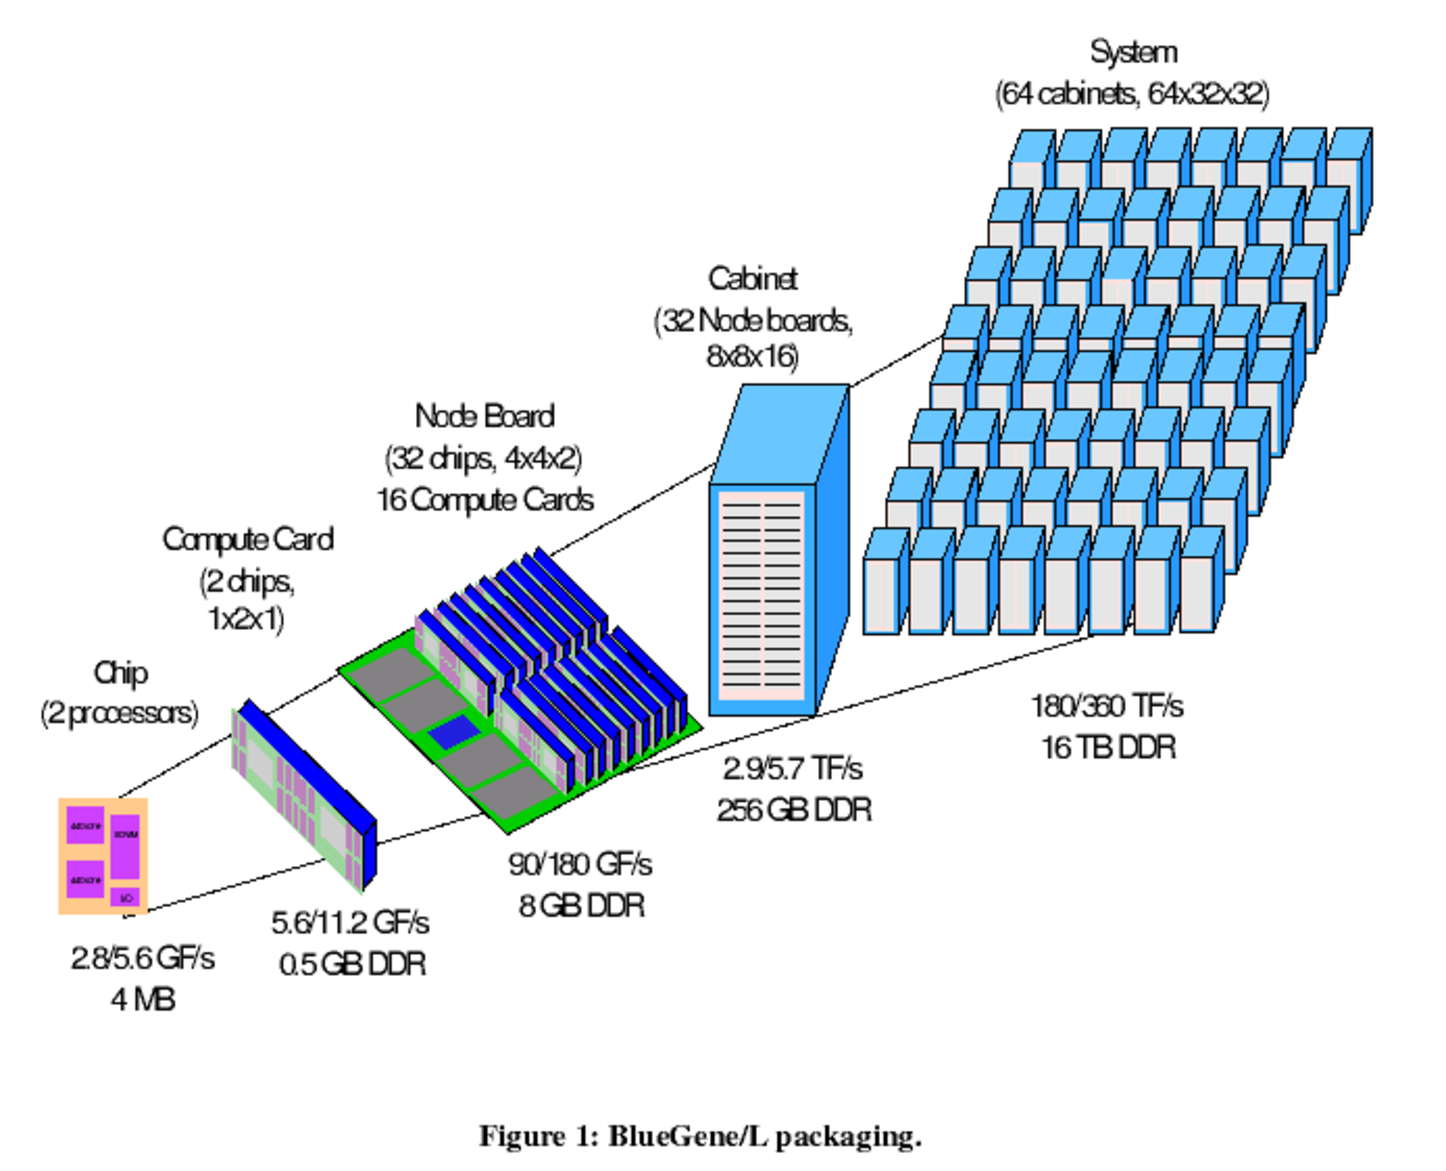
\includegraphics[width=.5\textwidth]{bluegenearch.pdf} 
\caption{\label{bglarch}Blue Gene System View.}
\end{figure}

The system we are currently using, the Blue Gene/P system at Argonne National Labs, has 40,000 Power PC 450 CPUs, 
with four cores and 2 Gbytes of memory each (for a total of 80 TB of memory). The memory is not globally addressable; communications are entirely via message passing. 
There are two CPU classes, I/O and Compute. What distinguishes the two types is their network connectivity. I/O nodes connect
to three networks: a 10 Gbit/second Ethernet, a 2.4 Gbit/second collective network which has a tree-like topology, and
a JTAG network for control and booting. The Compute nodes are attached to a 3D toroidal mesh network with six links per compute node and 500 MBytes/second bandwidth on each link.  The compute nodes are also connected to the collective, or "tree", network, and the JTAG network. The only connection between CPU nodes and I/O nodes is the tree network. The tree network is used for both computation support (CPU nodes only) and I/O (CPU node to I/O node communications). The I/O nodes, as the name implies, perform file system I/O as proxies for the 
compute nodes. For further detail the reader is referred to \cite{plan9bgp}. 

Currently, Blue Gene systems run two different kernels. The I/O nodes run Linux. The compute nodes run a lightweight kernel, the Compute Node Kernel or CNK.The CNK does not support file I/O directly; instead, system calls are packaged and forwarded to the I/O node. Experimentation with running Linux on the compute nodes is ongoing. 

\subsection{Plan~9}
Plan~9\cite{Plan9} is a distributed operating system developed at Bell Labs. In Plan~9, the only components hardwired into the kernel are those which are absolutely necessary for basic operations (drivers); other components, which can be on the same or other computer, are run outside the kernel (servers). Drivers include hardware controllers, process management, and network protocol stacks. Servers include traditional functions such as file systems and nontraditional functions such as window managers and Grid management tools. Drivers and servers can be transparently intermixed and their location is irrelevant; a server can be reimplemented as a driver with little if any code changing (the TCP/IP stack was originally a server but was moved into the kernel as a driver).

\subsection{Why Plan~9?}
Plan~9 was originally proposed by us as a "third way" between two alternatives: light-weight kernels (LWKs) which did not do quite enough -- on the Cray XT series, for example, the Catamount Light Weight Kernel does not support sockets or multiple processes -- and heavyweight kernels such as Linux. Measurements using the Fixed Time Quantum\cite{ftq} benchmark showed that a full desktop Plan~9 system had less OS noise than a single-user Linux system. Further, while Linux had far more features than needed, it lacked some key features that we wanted, the most important being support for dynamic user configuration of the node. We felt the proper way to provide this functionality was via a minimal, fixed-function kernel which could be extended by the \textit{user}, not the sysadmin, and \textit{during application execution}, not only at system boot time. 

For kernel properties fixed at build time, we wanted the ability to easily change such fundamental system parameters as page size. The Plan~9 hardware memory management code is one file; in most Unix systems it is several dozen (e.g. 55 in Linux). As related in \cite{plan9bgp}, adding huge pages to Plan~9 consumed less than 50 lines of code. 

%One of the single most contentious discussions in HPC in the last 20 years has revolved around the issue of "OS Bypass" 
%
%"OS Bypass" refers to the (now common) practice of embedding hardware device drivers for networks directly in the runtime library, usually MPI. OS bypass has been taken for granted in HPC for almost two decades. In essence, device drivers are moved from the kernel to the MPI library. As we have learned over the years, one end result is the recreation of a great deal of kernel functionality in the runtime libraries; nothing comes for free. In a sense, OS Bypass is the network of equivalent of how X11 uses graphics cards; just as X11 bypasses the kernel and drives the card directly, so OS Bypass drives a network card directly. The problems are much more complex on OS Bypass networks, since the user level software must manage all DMA directly, and the cards are either single user devices or must support virtual network card instances. 
%
%One of the goals of our work has been to reexamine OS Bypass. This reexamination is driven by the observation that kernels are typically very good at concurrency and allocation of resources; applications are good at computing; runtimes are good at interfacing the two. When runtimes start to take on tasks that are rightly part of the OS, trouble ensues as the kernel and the runtimes try to work around each others needs and, worse, duplicate functions and code. 
%
%Part of our work is to determine whether, given a sufficiently lightweight, efficient operating system, applications might do better to ask the kernel to move data, rather than moving data directly with a user-level device driver. 
%\subsection{Global Barrier}
%The global barrier hardware on Blue Gene supports four one-wire global networks. Each network supports a global \textit{and} or global \textit{or}; only one function (\textit{and} or \textit{or}) can be used on one network at a time. The CNK API is based on memory access: programs read and write the registers directly. This apparent low-latency access to the "bits on the wire"  is belied by the large body of library code actually placed between the program and the collective. 
%
%We implemented the barrier as a Plan~9 device with eight files: /dev/gib\{0-3\}barrier, and /dev/gib\{0-3\}intr. The barrier is a global \textit{and}, and the intr is a global \textit{or}; its name also indicates its role as an interrupt generation source. 
%
%A write system call to one of the barrier files blocks until all other nodes have written to the file, at which point it returns. The barrier file can not be read. A write system call to one of the intr files sets the global or line, which can be read by a read system call. 
%
%By implementing barriers this way, we make them availble to all programs, not just CNK binaries or programs that know how to directly control the barrier hardware registers. We can even use the barriers in shell scripts. For example, if we wish to have all nodes stop at some point in bootup and wait until all other nodes are ready, we can put this command in the shell script: 
%
%\texttt{echo 1 $>$ /dev/gib0barrier}

\section{Blue Gene networks and the OS Bypass question}
An early Blue Gene design decision was that  compute node applications would have direct user access to most network interfaces, i.e., the operating system would play no role whatsoever in moving data from program to program. The application, following the OS Bypass model, manages all aspects of the network, including DMA, interrupt handling, and limited error management (any real errors, such as packet loss, are unrecoverable and require a reset). 
We show a simplified version of the normal path in Figure \ref{ospath}, and an OS Bypass example in Figure \ref{osbypass}.
\begin{figure}
\includegraphics[width=2.5in]{ospath}
\caption{\label{ospath}The common OS path for I/O}
\end{figure}
\begin{figure}
\includegraphics[width=2.5in]{osbypass}
\caption{\label{osbypass}An OS Bypass example.}
\end{figure}
The kernel driver is disabled, or, in some cases, removed or never even written; the functions of the driver are replaced by 
an application or library. 
All HPC systems in the "Top 50",
%\cite{top500}, 
and in fact most HPC systems in the Top 500, use OS bypass. 

OS Bypass is the network equivalent of what systems such as X Windows do for graphics. 
As the name implies, the OS is completely bypassed; packets move only at the 
direction of the application. This mode of operation is a lot like the very earliest
days of computers, where not a bit of I/O moved unless the application
directly tickled a bit of hardware. It involves the application (or libraries) in the
lowest possible level of hardware manipulation, and even requires
application libraries to replicate much of the operating systems
capabilities in networking, but the gains are seen as worth the cost.

Why OS Bypass? Is OS bypass for HPC networks still needed, or might it be an anachronism driven
by outdated ideas about the cost of using a kernel for I/O?
The answer depends on measurement. There is not much doubt about the kernel's ability to move
data at the maximum rate the network will support; most of the questions have concerned the amount of 
time it takes to get a message from the application to the network hardware. 
So-called short message performance is crucial to many applications. 

HPC network software performance is frequently characterized in terms of "bits to the wire" (BTW) and "ping-pong latency". 
Bits to The Wire is a measure of how long it takes, 
from the time an application initiates
network I/O, for the bits to appear on the physical wire. Ping-pong latency 
is time it take a program to send a very small packet (ideally, one bit) from 
one node to another, and get a response (usually also a bit). 
These numbers are important as they greatly impact the performance of collectives (such as a global sum), 
and collectives in turn can dominate application performance\cite{petrini}\cite{ 10.1109/HPC.1997.592137}\cite{quadrics}.
In an ideal world, ping-pong latency is four times the "bits to the wire" number. 
Some vendors claim to have hit the magical 1 microsecond ping-pong number, but a more typical 
number is 2-3 microseconds, with a measured BTW number of 700 nanoseconds\footnote{This number has stayed 
remarkably constant for several decades, indicating that the systems have hit some fundamental limit, even as the processors 
have gotten 100 times faster. }.
However, these numbers always require dedicated hosts, devices
controlled by the application directly, no other network activity, 
and very tight polling loops. The HPC systems are turned into dedicated network benchmark devices -- really, dedicated marketing devices. 

%Unlike newer Inifiniband network interfaces, 
%Blue Gene does not provide a virtualizing network interface, i.e., only one application at a time may use the network. 
%Hence, the Blue Gene HPC network is a single-user device. Because one application 
%owns the network, that network becomes unusable to any other program or to the kernel. 
%This exclusivity requires, in turn, that all
%HPC systems be provisioned with several networks, increasing cost and decreasing reliability. While the reduction in reliability is not obvious, one must consider 
%that the two networks are not redundant; they are both needed for the application
%to run. A failure in either network aborts the application. Additional hardware has made the system less reliable. 

\subsubsection{How a non-OS Bypass program can use a kernel interface: synchronizing Blue Gene with a shell command}
Our implementation of a device interface to the BG/P global barrier shows an alternative to OS Bypass.
The global barrier hardware on Blue Gene supports four one-wire global networks. Each network supports a global \textit{and} or global \textit{or}; only one function (\textit{and} or \textit{or}) can be used on one network at a time. 

The global barrier on the Blue Gene systems is normally only 
available to programs that link in the Deep Computing Messaging Facility (DCMF) library or the 
MPI libraries\footnote{MPI libraries are typically much larger than the Plan~9 kernel; indeed, the configure script for OpenMPI is larger than the Plan~9 kernel.}, which in turn 
link in the DCMF. In the standard environments,  programs using the  HPC network must be written as an MPI 
application. The apparent low-latency access to the "bits on the wire"  is belied by the large body of library code actually placed between the program and the collective. 
Also, any program wishing to use the network must be rewritten as an MPI program, which is quite a limitation. 

The Plan~9 global barrier device provides access to the barrier network via eight device files: /dev/gib\{0-3\}barrier, and /dev/gib\{0-3\}intr. The barrier is a global \textit{and}, and the intr is a global \textit{or}; its name also indicates its role as an interrupt generation source. 
A write system call to one of the barrier files blocks until all other nodes have written to the file, at which point it returns. A write system call to one of the intr files sets the global or line, which can be read by a read system call. 
The device allows us to use the barriers in very non-traditional ways, even in shell scripts. For example, if we wish to have all nodes stop at some point in bootup and wait until all other nodes are ready, we can put this command in the shell script: 

\texttt{echo 1 $>$ /dev/gib0barrier}

By providing the network to programs as a kernel device, rather than a set of direct-access raw registers, we are making HPC usable 
to more than just specialized  MPI programs. While this uniform and clean model is attractive to computer scientists, it will only be acceptable to HPC users if there is a low latency path available to programs that need it; 
in other words, a path that equals OS Bypass performance must be available. HPC programmers are willing to go to some extra programming effort to use this path, but it 
{\em must} be there. 

\subsubsection{Seperating Implementation from Usage}
Making network resources available as kernel-based files
makes them more accessible to all programs. Separating the 
implementation from the usage  reduces the chance that simple application bugs will lock up the network. 
For example, the four global barrier networks are all controlled from one 32-bit register; simple programming bugs can result in the wrong barrier 
being used on some nodes. The Plan 9 devices makes it much harder for such errors to happen. 
Interrupts, errors, resource conflicts, and sharing can be managed by the kernel. That is why we developed kernels in the first place. 
But if these benefits come at too high a cost in performance, then we will have to give up 
on using the kernel devices and forfeit this elegant model. The reason to use OS bypass is the cost of asking the kernel to 
perform network I/O. 

One might think that the Plan~9 drivers, in order to equal the performance of OS bypass, need to impose a very 
low overhead -- in fact, no overhead at all: how can a code path that goes through the kernel possibly equal an
inlined write to a register? One must consider the real cost of the operation once the libraries have been taken into account.
It is true that the OS has been removed. But the need for thread safety and safe access to shared resources can not be removed: the support  has to go {\em somewhere}. That somewhere is the runtime library, in user mode. In fact even the most simple operations in the libraries take several thousand cycles. 

Hence, while it is true that OS bypass has near-zero overhead in theory, it has much higher overhead in fact. 
Programs that use OS bypass always use a library; the library is usually threaded, with a full complement of locks; 
OS functions are now in a library. In the end, an OS which compete with OS Bypass  has merely to offer lower overhead than the library. 

There are security problems with OS bypass as well. 
To make OS bypass work, the kernel must provide interfaces that to some extent break the security model. On Blue Gene/P, for 
example, DMA engines  are made available to programs  that allow them to overwrite arbitrary parts of memory. On Linux HPC clusters, 
Infiniband and other I/O devices are mapped in with mmap, and users can activate DMAs that can overwrite parts of kernel memory. Indeed, 
in spite of the IOMMUs which are supposed to protect memory from badly behaved user programs, 
there have been recent BIOS bugs that allowed users of virtual network interfaces to roam freely over memory above the 4 gigabyte
boundary\cite{iommubug}. Mmap and direct network access are  really  a 
means to an end; the end is low latency bits to the wire, not direct user access. It is so long 
since the community has addressed the real issue that means have become confused with ends. 

\section{Related work}
The most common way to provide low latency device I/O 
to programs is to let the programs take over the device. 
This technique is most commonly used on graphics devices. Graphics devices are inherently single-user devices, with multiplexing 
provided by programs such as the X server, which is designed to facilitate multi-user access to a single-user resource. 

Network interfaces, by contrast, are usually designed for operating systems kernels to manage. 
Direct access requires that the network be dedicated to one program. Multi-program access is simply impossible with 
standard networks. In contrast with the X server, OS Bypass is designed to provide single-user control of a network resource. 
The means are similar, the ends entirely different. 

Trying to achieve high performance while preserving multiuser access
to a device has been achieved in only a few ways. In the HPC world,
the most common is to virtualize the network device, such that a
single network device appears to be 16 or 32 or more network
devices. Such devices consume a great deal of power: a typical
low-power 40 Gbit/second Infiniband interface consumes 5 Watts; a full
BG/P node card including DRAM consumes 17 Watts; providing 5 Watts
just to a network interface is an unacceptable proposition. Further,
these cards require either a complex hardware design or a
microprocessor running a real-time operating system: thus, the
complex, microprocessor-based interfaces do bypass the main OS, but
don't bypass the on-card OS\cite{Boden95myrinet}.  These devices are
usually used in the context of virtual machines. Device virtualization
requires hardware changes at every level of the system, including the
addition of a so-called iommu\cite{iommu}.

An older idea is to dynamically generate code as it is needed. For example, the code to read a certain file can 
be generated on the fly, bypassing the layers of software stack. One implementation of this idea 
is found in   Synthesis\cite{synthesis}. While the approach is intriguing, 
it has not proven to be practical, and the system itself was not widely used. 

The remaining way to achieve higher performance is by rigorous optimization of the kernel. Programmers
create hints to the compiler, in every source file, about the expected behaviour of a branch; locks are removed; 
the compiler flags are endlessly tweaked. In the end, this work results in slightly higher throughput, but the 
latency -- "bits to the wire" -- time changes little if at all. It is still too slow. Recent experiences show that 
very high levels  
of optimization can introduce security holes, as was seen when a version of GCC 
optimized out all pointer comparisons to 
NULL. 

Surprisingly, there appears to have been little other work in the area. The mainline users of operating systems do not care; they consider 1 millisecond 
BTW to be fine. Those who do care use OS bypass. Hence the current lack of 
innovation in the field: the problems are considered to be solved. 

The status quo is unacceptable for a number of reasons. Virtualized device hardware increases costs at every level in the I/O path. Device
virtualization 
adds a great deal of complexity, which results in bugs and security holes that are not easily found. The libraries which use these 
devices have taken on many of the attributes of an operating system, with threading, cache- and page-aligned resource allocation, 
and failure and interrupt management. Multiple applications using multiple virtual network interfaces end up doing the same work, with the same
libraries, resulting in increased memory cost, higher power consumption, and a general waste of resources all around. In the end, the applications 
can not do as good a job as the kernel, as they are not running in privileged mode. Applications and libraries do not have access to
virtual to physical page mappings, for example, and as a result they can not optimize memory layout as the kernel code. 

\section{Currying and Process Private System calls}
We first provide an overview of file I/O in Plan 9, to better explain our changes. It is similar to the Unix-compatible OSes such as the various BSDs and Linux, 
but at the same time there are enough differences to make an outline useful. 

Processes perform I/O with only two system calls, read and write. As on all Unixes, I/O is initiated by a system call trap. 
The kernel then takes the following steps:

\begin{itemize}
\item Validate the system call number.
\item Call the system call function. From this point on we will only consider the the read/write functions. 
\item Assemble arguments. Arguments are pulled from the stack, which involves a copyin. Register parameters are used in only a limited way in Plan~9. 
\item validate the (integer) file descriptor, convert it into an internal pointer to a channel (i.e. file) struct and increment the usage lock to ensure the channel is not closed while in use. 
\item Validate the memory region and access mode. The semantics of write require that the process block 
until the data is completely used, or that the process not be able to change the data once the write call returns (i.e. 
the semantics do not allow asynchrony). Some Unix systems support asynchrony by fiddling with the 
page attribute bits, ensuring that post-system-call changes occur in a different page. Others copy data to an internal buffer. Others block the process until the data is no longer needed. 
In keeping with the goal of simplicity, Plan~9 copies the data to or from an internal structure called a {\em qio}. Qio structs form a linked list. The kernel dequeues write data and may coalesce it into large chunks, and similarly enqueues read data. The data copy always occurs in the process virtual memory context. 
\item Indirect through the channel structure members to call the driver write function
\item On return, manage any errors and unlock the channel. 
\item Set up return results and copy out data if necessary
\end{itemize}

In most cases, the steps outside the actual I/O itself are not expensive relative to the actual I/O. If the write involves
sending packets over a network, or writing a disk, the file descriptor and address validation are insignificant, a few microseconds at most. The picture changes completely with a slow processor (as the PowerPC 450 is) and a fast network, as we have on Blue Gene. Then, the overhead of setting up the arguments alone can dominate the overall time. A global barrier operaion across 65536 nodes can be done in 125 nanoseconds 
on Blue Gene; that is 106 instructions. Each instruction takes 1.2 nanoseconds; it does not take long to double the time to run a global barrier. 

As can be seen above, there is a lot of repeated work for each system call. It is reasonable to ask just how much the arguments vary for each write system call. How much of this work is unneccesary because we are validating the same parameters, over and over? 
We instrumented the Plan~9 kernel and monitored 
applications using  a trace device\cite{iwp9:tracedevice}. We measured all the I/O performed by all processes over 
a 30 minute interval. We learned that, in general, programs read and write a small 
set of files over and over, from a very small set of virtual addresses, with a very limited and small range of sizes. This result makes intuitive sense: consider programs on Unix which use stdio, for example: file I/O is performed 
to an internal buffer which does not change, and the buffer size is usually limited to a page size or smaller. Other I/O addresses are almost always from the stack (i.e. an auto variable). Our measurements confirmat this intuition, at least for Plan~9. 

We also learned that the bulk of the time for basic device I/O with very small write sizes -- the type of operation common to collective operations -- was taken up in two functions: the one that validated an open file descriptor, and the one that validated an I/O address. 
The measurements indicate that we could benefit from caching active file descriptors and virtual address ranges in each process structure. Caching virtual to real translation information for just 32 address ranges would eliminate all page table walks for almost all process I/O. Caching just 8 file descriptors would eliminate almost all file descriptor validation operations. Of course, this caching would not cover some extreme cases (Apache), but it would cover the most common. 

%The basic I/O path and opportunities for caching are shown in Figure \ref{caching}.
%\begin{figure}
%\caption{\label{caching}Plan~9 I/O path and caching opportunities
%\end{figure}

At the same time, such caching adds a level of complexity that is not consonant with the structure of the Plan~9 kernel. Caches must be validated and cleaned. There would be interactions with other processes and the virtual memory subsystem. Callbacks would be needed when a process forked or exited to make sure cached file descriptors are managed. 

While we considered the caching approach, we eventually rejected it for two reasons. The first was the complexity and the opportunity for introducing bugs. The second was that it might increase the amount of code being run, or at the least not decrease it enough. What we need is a system call interface that eliminates almost all of the kernel code save the actual driver I/O steps -- we want to do a type of OS bypass, but after the OS has been entered. What we want is to bypass all the generic system call code and get right to the business of performing actual I/O. 

Our approach is a modification of the Synthesis approach. We do create curried functions with optimized I/O paths, 
\begin{figure}
\includegraphics[width=2.5in]{curry}
\caption{\label{curry}Our approach: in-kernel OS Bypass}
\end{figure}
but we do not generate code on the fly; curried functions are written ahead of time and compiled with the kernel, and only for some drivers, not all. The decision 
on whether to provide curried functions is determined by the driver writer. 
This approach can be thought of as an {\em in-kernel OS Bypass}. While programs must still switch to the OS to do the I/O, much of the standard OS processing is bypassed, since it is done ahead of time. 

At run time, if access to the curried function is requested by a program, 
the driver  pre-evaluates and pre-validates arguments and sets up the parameters for the driver-provided curried function. 
Commands are written to the {\tt ctl} file of the driver to set up the fast path. 
The 
curried function is made available to the user program as a private system call, i.e. the process structure for 
that one program is extended to hold the new system call number and parameters for the system call. 
Thus, instead of actually synthesizing code at runtime, we augment the process structure so as to 
connect individual user processes to curried 
functions which are already written, with a customized set of parameters contained in a struct attached to the proc structure. 

We have achieved sub-microsecond system call performance with these two changes. The impact of the 
changes on the kernel code is quite minor. 

We will first digress into the nature of Curry functions, describe our changes to the kernel and, finally discuss the 
performance improvements we have seen. 

\subsection{Currying}
The technique we are using is well known in mathematical circles, and is called currying. 
We will illustrate it by an example. 

Given a function of two variables, $ f\left( x, y\right) = y/x$, 
one may create a new function, $g\left( x\right)$, 
if $y$ is known,  such that $g\left( x\right) = f\left( x, y\right)$. 
For example, if y is known to be 2, the function g might be $g\left( x\right) = f\left( x, 2\right)$. 

We are interested in applying this idea to two key system calls: read and write. Each takes a 
file descriptor, a pointer, a length, and an offset. 

The application of currying was obvious: given a program which is calling a kernel function read or write function: $ f\left( fd, address, size\right) $, with 
the same file descriptor and same address, we ought to be able to make a new function: 
$g\left( size\right) = f\left( fd, address, size\right)$, or even 
$g\left( \right) = f\left( fd, address, size\right)$. 

Tracing indicated that we could greatly reduce the overhead. Even on an 800 Mhz. Power PC, we could 
potentially get to 700 nanoseconds. This compares very favorably with the 125 ns it takes the hardware to actually
perform the global barrier (that time is included in the 700 ns.).

\subsection{Connecting curry support to user processes}
The integration of curried code into the kernel is a problem. 
Dynamic code generation looks more like a security
hole than a solution. 

To support Currying without dynamic code generation, the kernel is extended: 
\begin{itemize}
\item extend the process structure to contain a private system call array, used for creating curried system calls
\item extend the system call code to use the private system call array when it is passed an out-of-range system 
call number
\item extend selected drivers to accept a  command to create the curried system call
\item extend the driver to provide the curried function. The function uses only pre-validated arguments from the private system call entry structure
\end{itemize}

\section{Implementation of private system calls on Plan~9 BG/P}
To test the potential speeds of using private system calls, a system was implemented to allow fast writes to the barrier network, specifically for global OR operations, which are provided through {\tt /dev/gib0intr}. The barrier network is particularly attractive due to its extreme simplicity: the write for a global OR requires that we write to a 
Device Control Register, a single instruction, which in turn controls a
wire connected to the CPU. 

The data structure for holding pre-validated arguments is shown in Figure \ref{scstruct}. Since there are only two I/O calls on Plan~9 this structure covers all uses of currying. 

\begin{figure}
\begin{verbatim}
struct Fastcall {
	/* System call number */
	int	scnum;
	/* File */
	Chan*	c;
	/* Function */
	void	(*fun)(Ar0*, Fastcall *);
	/* Pre-validated arguments */
	void*	buf;
	int	n;
	vlong	offset;
};
\end{verbatim}
\caption{\label{scstruct}Fast system call struct}
\end{figure}

To set up the private system call, programs are required to provide a system call number, a file descriptor, pointer, and length.

The Blue~Gene barrier device is extended to accept {\tt fastwrite} as a command when written to {\tt /dev/gib0ctl}\footnote{Plan~9 has no {\tt ioctl} system call; for all devices, ioctl-like commands 
are written as text to a device file, by convention called ctl.}. When the command is written, the kernel allocates a new {\tt Fastcall} and attaches it to the proc structure. The code to set up the fast path is shown in Figure \ref{code}.
\begin{figure}
\begin{verbatim}
int cfd, gdf, scnum=256;
char area[1], cmd[256];
gfd = open("/dev/gib", ORDWR);
cfd = open("/dev/gib0ctl", OWRITE);
cmd = smprint(
  "fastwrite %d %d 0x%p %d", 
  scnum, fd, area, sizeof(area));
write(cfd, cmd, strlen(cmd));
close(cfd);
docall(scnum);
\end{verbatim}
\caption{\label{code}Sample code to set up a curried systemcall}
\end{figure}

Following the {\tt write}, {\tt scnum} contains a number for a private system call to write to the barrier network. From there, a simple assembly function (here called {\tt docall}) may be used to perform the actual private system call. The code is shown in Figure \ref{docall}. The compiler is caller-save on Plan~9. It places the first parameter (in this case the private system call number) in {\tt R3}, and the return is in {\tt R3}, so
the code is quite minimal. 

\begin{figure}
\begin{verbatim}
TEXT docall(SB), 1, $0
    SYSCALL
    RETURN
\end{verbatim}
\caption{\label{docall}User-defined system call code for Power PC}
\end{figure}

When a system call interrupt is generated, the kernel typically checks
if the system call number matches one of the standard calls; if there
is a match, it calls the appropriate handler, otherwise it gives an
error. However, the kernel now also checks the user process's private
system call set and calls the curried function call if a matching
private call exists. In the case of the barrier device, it calls the
curried write function for the barrier. The curried call avoids several
layers of generic code and argument checking, allowing for a far
faster write.

\section{Results for two networks}
\subsection{Global Barrier Network}
We achieved our goal of sub-microsecond bits to the wire. With the traditional write path, it took approximately 3,000 cycles per write. Since the BG/P uses 850 MHz PowerPC processors, this means a normal write takes approximately 3.529 microseconds. However, when using the private system calls, it only takes around 620 cycles to do a write, or 0.729 microseconds. The overall speedup is 4.83. 
The result is a potential ping-pong performance of slightly under 3 microseconds, which is competitive with the best OS bypass performance. 

\subsection{Torus Network}
The Torus network consists of a 3D toroidal mesh with 6 500 Mbyte/second links. Packets consist of one or more 
256-byte fragments, of which 240 bytes are available for user data. Sending larger packets involves queueing up multiple smaller packets, but a remote DMA and scatter/gather support are available. 

The Plan 9 performance for one direction time was 25 microseconds, round trip time was a bit over 50. These times do not compare well to MPI; they are 12 times slower than an MPI ping\cite{1375544}, which with small messages and two nodes runs in about four microseconds. In fact the authors of \cite{1375544} point out that were MPI not used, they could remove a further 2.2 microseconds of overhead from the ping. The Plan~9 performance on the Torus is simply not competitive. 

We created a non-MPI ping program and modified the kernel so we could follow a packet in time as it
traversed the kernel and the two programs. We recorded the Power PC Time Base Register into the
packet as it made the transition from local kernel to remote kernel and back again. Given a 64-bit
time base, the shortest packet can contain 30 time stamps for different points in the path; we used
28 of them. The results are shown in Figure  \ref{pingpongcurry}. The coloring shows first the transmit-side in red; the remote receive side in green; the remote response (send) side in purple; and the local receive side in blue. The names of the points and their meaning are shown in Table  \ref{pingnames}. What the graph shows are 100 consecutive trials, with the time for each. There is very little variation in the times, which is a good sign; however, the times themselves are quite long.
 \begin{figure}
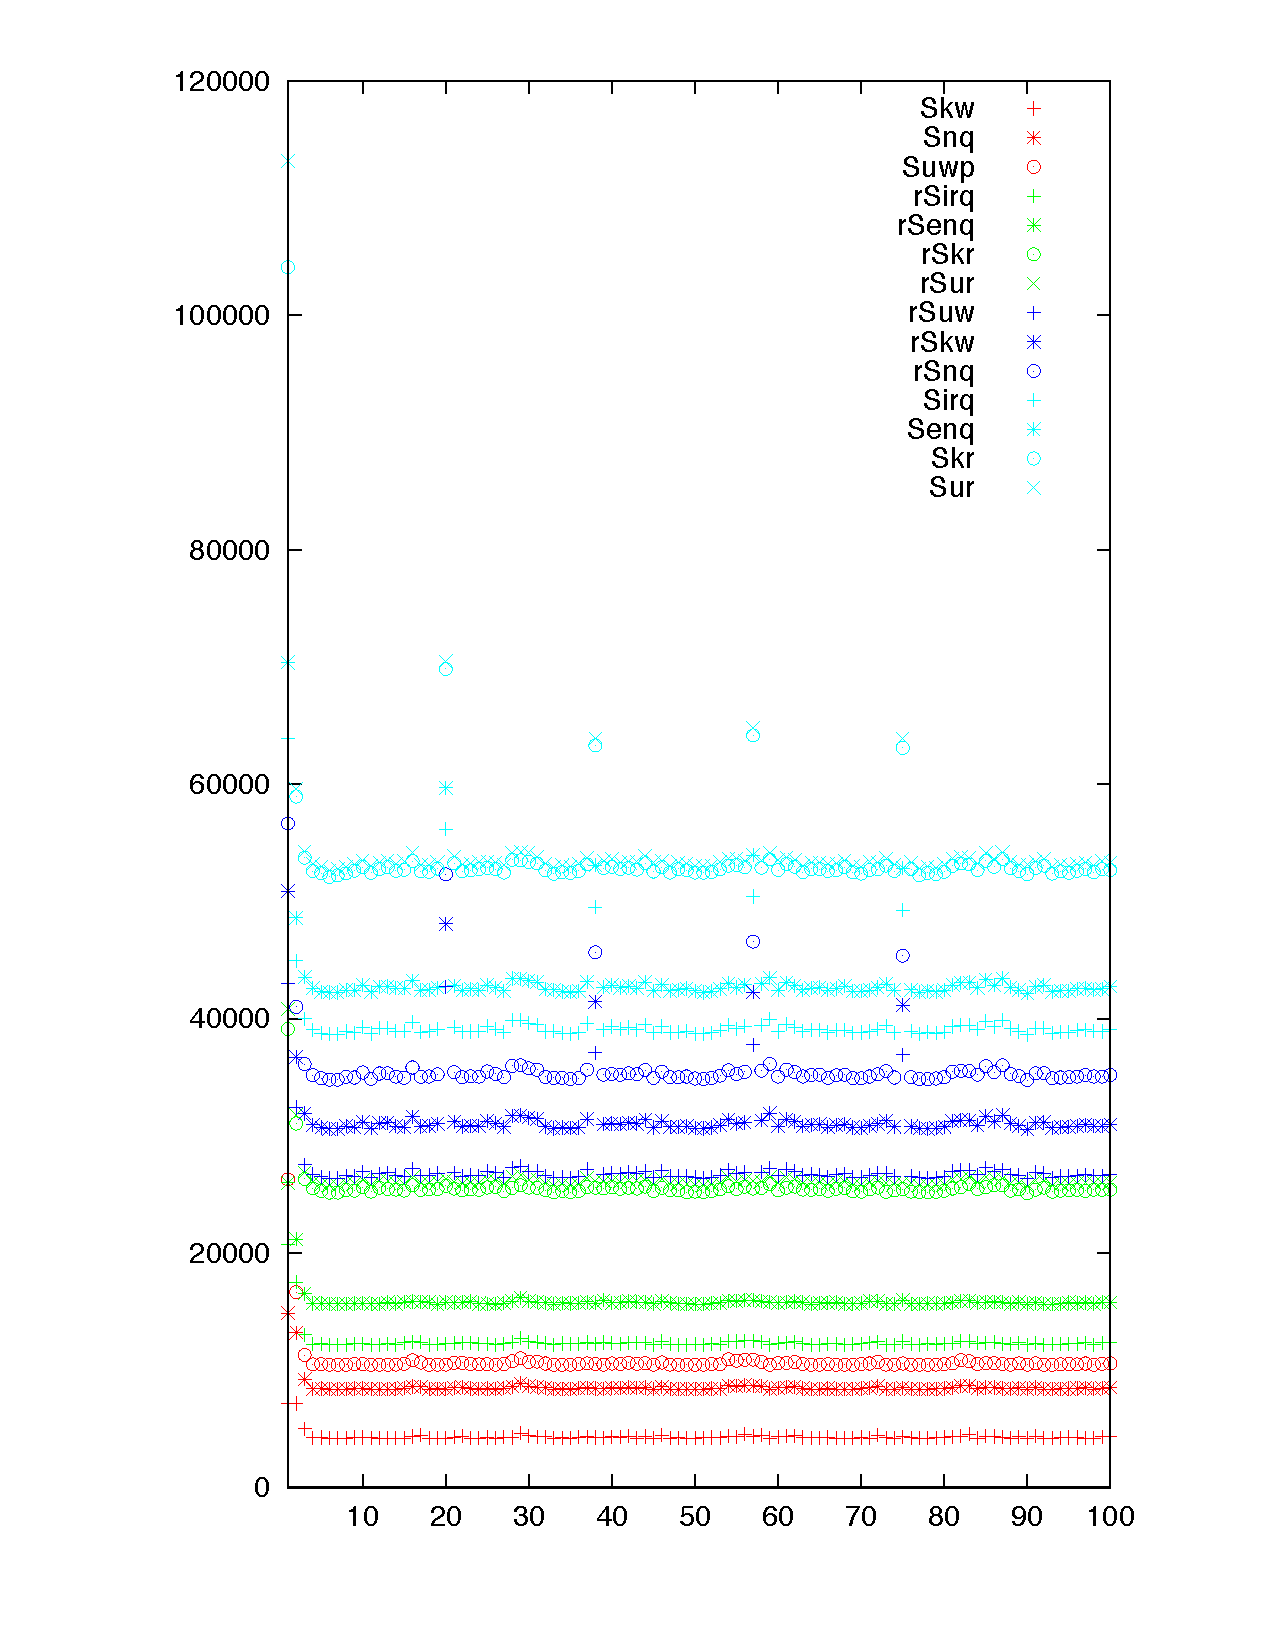
\includegraphics[width=.5\textwidth]{pingpongcurry.pdf} 
\caption{\label{pingpongcurry}Performance for a ping packet as it traverses user program, kernel, and network.}
\end{figure}

\begin{table}[ht]
\centering
 \begin{tabular}{c p{2.5in}} \hline\hline Name & Meaning \\ \hline
 Skw & Entry point for curried kernel write system call \\ \hline
 Snq & Top of function for enqueueing the Torus packet \\ \hline
 Suwp & Point at which packet is written to the hardware \\ \hline
 rSirq & Entry point for remote Torus receive interrupt \\ \hline
  rSenq & Torus receive enqueue function \\ \hline
  rSkr & Exit point for kernel read function \\ \hline
  rSur & Return to remote user ping from kernel \\ \hline
  rSuw & Remote user mode write \\ \hline
  rSkw & Remote entry pint for curriend kernel write system call \\ \hline
  rSnq & Remote enq \\ \hline
  Sirq & Local Receive IRQ \\ \hline
  Senq & Local enqueue for read system call \\ \hline
  Skr & Return to user mode from kernel \\ \hline 
  Sur & Local user mode for read, i.e. end of one ping cycle
  \end{tabular}
\caption{\label{pingnames}Measurement points in the ping.}
\end{table}

Given the knowledge of what these times mean, we can see that the time on the network (seen as the transition from one color to another) is minimal. On each side, most of the time is spent between Sirq and Sur, i.e. between the receive interrupt and the kernel read system call handler. In fact the time from receive IRQ to user mode accounts for over 30 microseconds. 

A set of simple changes to the injection (i.e. transmit) side of the driver shaved 8 microseconds from the total time, 
reducing send overhead from 11 microseconds to 2.8. This time is still far too long, although it is better. 

Even if we improve the time on the write side, most of the time is consumed on the receive side. 
The problem is the traditional design of the Plan 9 driver and virtual memory architecture. As mentioned above, in Plan~9, data movement from the kernel to user process must be done in the virtual memory context of the user level process, using the qio structs. In other words, for the data to get to user mode, the user process must be scheduled and run. This design further requires the creation of queues: drivers push data into the queues, and processes pull it out. Hence, Plan~9 interrupt handlers must enqueue data and then schedule the user process, because only the user process (in kernel context) can copy the data to user mode. There are at least two copies and a call to malloc in the data path, and one is completely unavoidable. Given that in future machines power and bandwidth are even more of an issue than they are now, this design is clearly going to need to change. 

We might consider a fast path system call for the read operation as well, but it would require that we save user physical addresses in the driver, and ensure that the virtual 
to physical mapping for those addresses not change. That is not really an issue as Plan 9 does not implement swap and does not move pages around once they are mapped; once a user process has a memory page, the physical page does not change. 

\subsection{Discussion}
Currying worked well for the Barrier network, because there was so little I/O. There is no data transmission to speak of for the barrier. The data can be passed entirely in one register. Further, the process blocks in the write call, and returns when the barrier finishes; there is no need to call a read system call and wait to be rescheduled by an interrupt handler. 

The Torus results were not nearly as good as they need to be: at least a factor of 10 slower than the user-mode libraries. 
The experience suggests both that Plan~9 and the Torus interface need to be redesigned if we are to achieve our goals. 

The Torus interface is very deliberately designed to support one program at a time; that program being an MPI program which has three or four physically contiguous segments and which can compute the physical address for a virtual address trivially. The design, in other words, is entirely for user-managed, user-controlled, remote DMA on a system which never encounters failures and which is safe passing physical addresses to other programs on other nodes. While we had hopes that we might be able to modify Plan~9 to work well with this design, it is clear from our experience that the Torus may require too many changes. 

Remote DMA on the Blue Gene Torus can be thought of as a form of "super-currying". User-mode processes compute physical DMA addresses and pass them around the network. This mode of operation places many restrictions on the usage of Blue Gene. Only one process at a time can use the Torus. Any program which uses the Torus must be written to use MPI or the DCMF libraries. Failure is simply not allowed: a lost message, or one lost node out of 65536 nodes, requires a reboot. It is difficult to imagine that this model can scale well to future systems with millions of nodes. 
There is another factor to consider as well. Setting up an efficient path requires that applications pre-ship physical addresses to other nodes. These addresses almost always refer to 
memory chunks which are a page in size. On a system with one million MPI processes, such as the Sequoia system being built now, an all-to-all communications pattern would require 4 Gbytes of memory of the 16 Gbytes available to ensure that every sending process had a unique place for its packets to land. This huge resource commitment is not what is practiced; in fact, runtime libraries attempt to minimize the connectivity of the nodes. Because the Plan~9 implementation does not send physical addresses between nodes, this limitation
does not exist.

We can not completely lay the blame on the Torus, however. The Plan~9 I/O system is not adequate for modern hardware. The Plan~9 model is that user programs perform read and write system calls, and the data is copied from/to user mode and into a kernel mode data buffer. DMA operations are performed on kernel-owned IO buffers, not user buffers. Plan~9 nicely avoids the problems that come with using user memory addresses directly, which require virtual memory tricks to lock pages down while I/O is in progress; copy-on-write; and so on. While this design has brought a substantial reduction in virtual memory complexity, and a consequent improvement in reliability, at the same time it loses many opportunities to avoid copies. The problems are especially pronounced on the receive side, where zero-copy and fast switching to a receiving process are almost impossible. There are more issues with zero-copy than in previous years: extra copies consume power and starve cores of memory bandwidth. 

At the same time, it must be remembered it is possible to do zero copy in multiple ways and some of them are wrong for the newer NUMA CPUs. While the interrupt handler is running on one CPU, it is essential that the data be directed to memory attached to the  CPU on which the application is running. Per-core memory allocation pools are required. Page flipping, which was a very popular concept as little as 10 years ago, might work to implement zero-copy on Blue Gene today, but is the wrong solution for newer architectures. 

We would not want to copy the complexity of the Linux virtual memory
system to Plan~9. At the same time, there is a clear need for
significant change. For the Horizon supercomputer\cite{horizon} we had
contemplated an address space in which there were no unique addresses. 
Processes and the operating system would be provided with a single 
linear address space in which any virtual address was mapped uniquely 
to a physical address. Virtual memory hardware would still provide 
protection between processes, however. 
The
final step in loading a program for execution would have been to
relink it for its location in memory, much as Linux relinks kernel
modules when they are loaded today.  This so-called single address
space model has found more recent use in
Singularity\cite{singularity}. Such a model would allow transparent
sharing of data buffers between user and kernel processes, as well as
between processes on one machine. The single address space idea
becomes attractive each time the address space of the systems double
(i.e. from 16 to 32 to 64 bits) and there is far more virtual than
physical address space available; as physical memories expand, single
address space systems become less attractive. It seems that single
address space might work on 64-bit machines -- for now. It is one
alternative we are considering for the Plan~9 follow-on operating
system.

Still worse than the problem of data copies is the need to block and resume the process as I/O is performed. On a multicore system, it makes more sense for the process to have a lightweight mechanism to pause, but still remain sheduled on the core. Once the interrupt handler runs, it should be able to drop the data directly, with no copies, into the user buffer, and then resume the process without a heavyweight scheduling operating. We are also exploring these ideas. 

Finally, the question of the read/write interface needs another
look. Is there a system call that can be used to implement read/write,
but at the same time has extended semantics for our lower latency
requirements?

\section{Conclusions and Future Work}
Runtime systems for supercomputers have been stuck in a box for 20 years. The penalty for using the operating system was so high that programmers developed OS bypass software to get around the OS. The result was the re-creation of OS software above the operating system boundary, including support for device drivers, cache management, memory management, file system protocols, file servers, and many other functions we normally associate with an operating system. Only programs written to use the HPC libraries (which include a user-level device driver) could use the HPC networks, and only one program at a time could use them. Operating systems have been recreated as user libraries and, worse, they're single-user: HPC systems are little different that PCs running  DOS. Frequently, the performance of OS bypass is cited without taking into account the high overhead of these user-level operating systems, and the problems inherent in creating layers of redundant functions between the operating system and programs, much less the fact that only specially written programs can use the HPC network. 

This paper shows an alternative to the choice of slow operating systems paths or fast user-level operating systems paths. It is possible to use a general-purpose operating system for I/O and still achieve high performance in some cases. But, as always, the cost of process scheduling and data movement extract a penalty, and the combined problems of the network architecture and Plan~9 IO system design conspire to limit our performance as compared to the user-level approaches currently used on Blue Gene. 

We conclude in the end that both network interfaces and Plan~9 need to change if we are to make high performance network IO supported by the operating system, not user libraries. At the same time,we have also shown that in some cases, we can equal the performance of OS Bypass. The latency requirements traditionally associated with HPC are now becoming of importance to commercial HPC, such as trading platforms; it seems this issue must be addressed in a broader context than just HPC as it has been practiced. 

\section{Acknowledgements}
This work is support by the DOE Office of Advanced Scientific Computing Research. IBM has provided support from 2006 to the present. This research used resources of the Argonne Leadership Computing Facility
 at Argonne National Laboratory, which is supported by the Office of Science
 of the U.S.
 Department of Energy under contract DE-AC02-06CH11357.

\bibliographystyle{abbrvnat} 

\bibliography{all}

\end{document}
